\documentclass{article} 
\usepackage[utf8]{inputenc}
\usepackage{amsmath, amssymb, systeme, mathtools, lmodern, float, graphicx}
\usepackage[most]{tcolorbox}
\usepackage[scale=.95,type1]{cabin}
\usepackage[framemethod=tikz]{mdframed}


\usepackage[legalpaper,margin=1in]{geometry}

\setlength{\parindent}{10pt}
\setlength{\parskip}{1em}
\renewcommand{\baselinestretch}{1.2}

\title{Monoids and semigroups}
\date{}

\makeatletter
\renewcommand*\env@matrix[1][*\c@MaxMatrixCols c]{%
  \hskip -\arraycolsep
  \let\@ifnextchar\new@ifnextchar
  \array{#1}}
\makeatother

\newcommand\y{\cellcolor{blue!10}}

\usepackage{tabularray}
\SetTblrInner{colsep=5pt,rowsep=1pt}

\newcounter{Def}[section]
\newenvironment{Def}[1][]{%
  \ifstrempty{#1}%
  {\mdfsetup{%
    frametitle={%
      \tikz[baseline=(current bounding box.east),outer sep=0pt]
      \node[line width=1pt,anchor=east,rectangle,draw=blue!20,fill=white]
    {\strut \color{black}{Definition}~};}}
  }%
  {\mdfsetup{%
    frametitle={%
      \tikz[baseline=(current bounding box.east),outer sep=0pt]
      \node[line width=1pt,anchor=east,rectangle,draw=blue!20,fill=white]
    {\strut \color{black}{Definition}~:~\color{blue4}{#1}};}}%
  }%
  \mdfsetup{innertopmargin=2pt,linecolor=blue!20,%
            linewidth=1pt,topline=true,%
            frametitleaboveskip=\dimexpr-\ht\strutbox\relax,}
  \begin{mdframed}[]\relax%
  }{\end{mdframed}}
%{\fontfamily{cmtt}\selectfont }

\begin{document}
\section{Applicative laws}
Identity, composition, homomorphism, interchange.

\begin{Def}[Identity]

{\fontfamily{cmtt}\selectfont pure id <*> x}  
\end{Def}




\begin{Def}[Composition]
{\fontfamily{cmtt}\selectfont pure (.) <*> u <*> v <*> w}\\
  {\fontfamily{cmtt}\selectfont u <*> (v <*> w)}
  
\end{Def}



  
  \begin{Def}[Homomorphism]
    A \textit{homomorphism} is a structure-preserving map between 2 algebraic structures.
  \end{Def}

  \begin{Def}[Interchange]
    {\fontfamily{cmtt}\selectfont u <*> pure y = pure (\$ y) <*> u}
  \end{Def}

\begin{center}
  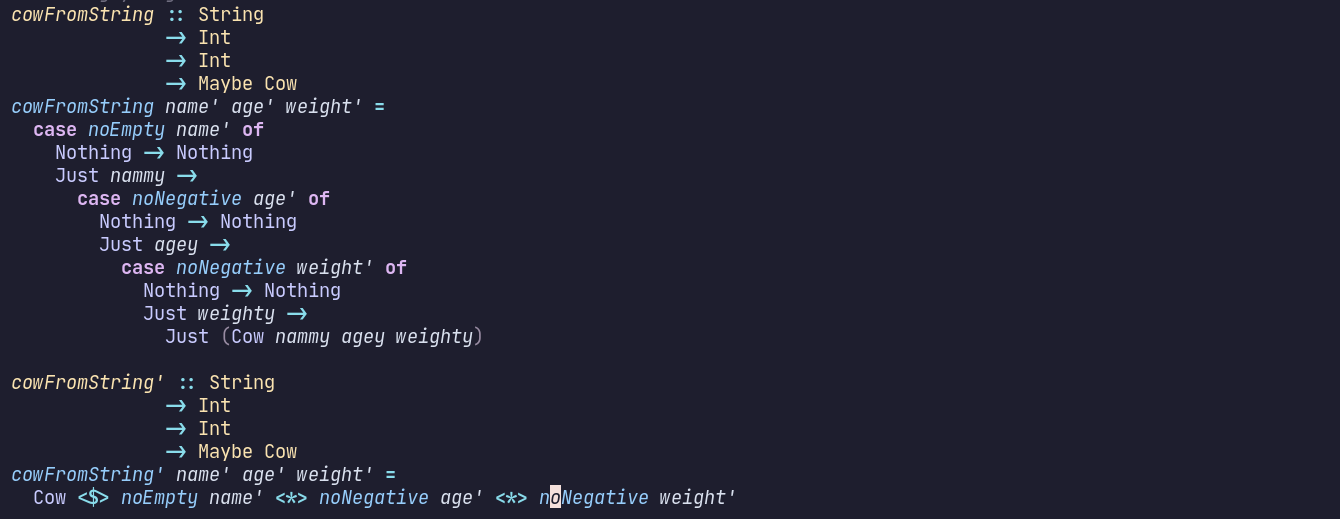
\includegraphics[width = \linewidth]{./cow.png} 
\end{center}
  
Validation, failure and success.
  
\section{Definition}
Applicative can be thought of characterizing monoidal functors. It's a way to functorially apply
a function embedded in structure $f$ of the same type as the value we are mapping over.
  
Note:
Idiom means applicative functor and is a useful search    term for published work on applicative functor.
\end{document}
